\section{Introduction}



% To address this challenge, we model workflows as sequences of LLM-invoking nodes connected by edges, representing all possible workflows, and frame automated workflow optimization as a search problem in a specific space. 

% To navigate this space, we present AFLOW, an automated framework for effective workflow search. AFLOW leverages Monte Carlo Tree Search to iteratively optimize nodes and edges within a predefined search space, utilizing tree-structured experience and execution feedback to derive effective workflows. 

% Empirical evaluations across six benchmark datasets demonstrate AFLOW's efficacy, yielding a 5.7\% average improvement over state-of-the-art baselines. Moreover, AFLOW enables smaller models to outperform GPT-4o on specific tasks at 4.55\% of the computational cost.

% ----- 第一段 -----
% Large language models (LLMs) have demonstrated remarkable potential in solving complex tasks across diverse domains, typically harnessed through agentic workflows comprising detailed instructions and operational sequences. However, creating these workflows demands significant human effort, limiting scalability and generalizability. 

Large Language Models (LLMs) have emerged as powerful tools for solving complex tasks across various domains, including code generation, data analysis, decision-making, and question answering~\citep{DBLP:journals/corr/abs-2408-05109, bo2024nlsql, DBLP:journals/corr/abs-2406-07815, yu2024hai, sun2024chatbot, wangchain, song2023llm, xietravelplanner, li2024debug}. However, the rapid advancement of LLMs heavily relies on manually designed agentic workflows -- structured sequences of LLM invocations accompanied by detailed instructions. Designing and refining these workflows requires significant human effort, which limits the scalability and adaptability of LLMs to new, complex domains and hinders their ability to transfer skills across diverse tasks~\citep{DBLP:conf/cidr/0001YF0LH24}.

Recent efforts have focused on automating the discovery of effective agentic workflows to reduce the reliance on human intervention~\citep{omar2024dspy, mert2024text,liu2023dynamic,hu2024automated}. Despite these advancements, full automation has not been achieved. For instance, \citet{omar2024dspy} requires manual workflow setup before automated prompt optimization. Similarly, methods proposed by \citet{mert2024text} and \citet{zhuge2024gptswarm} fail to capture the full diversity of workflows necessary for a wide range of tasks~\citep{yu2023thought, yang2024buffer, sun2023indeterminacy}, as their optimization objectives struggle to represent the breadth of possible workflows. The inability to effectively model diverse workflow structures within these automated systems limits their utility and impact.
ADAS~\citep{hu2024automated} represents workflows using code, achieving a relatively complete representation. However, due to the efficiency limitations of its linear heuristic search algorithm, ADAS struggles to generate effective workflows within a limited number of iterations. This highlights the need for more effective techniques to represent and automate the generation of agentic workflows, which would accelerate the application of LLMs across domains.

\begin{figure}[t!]
  \centering
  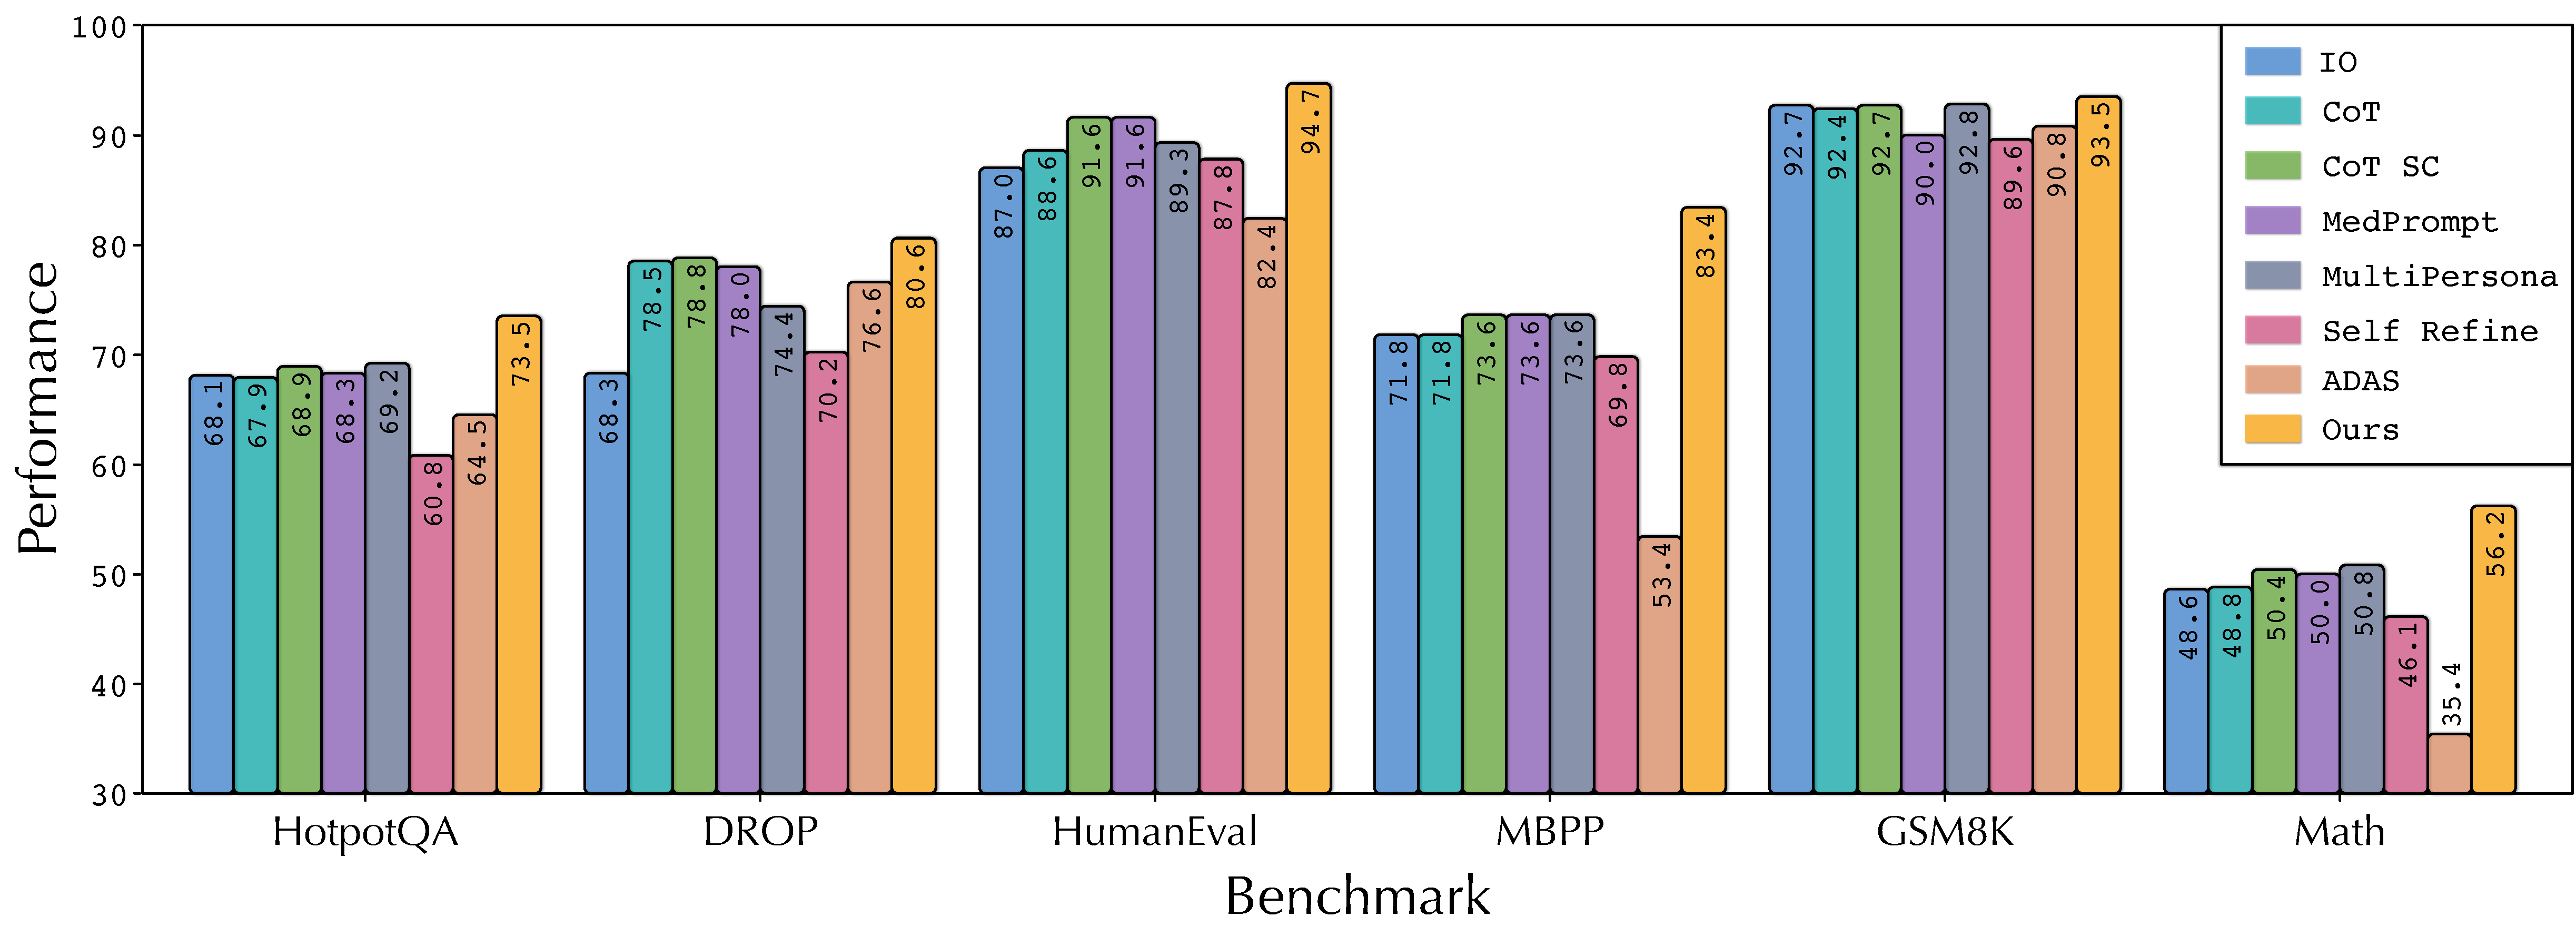
\includegraphics[width=\linewidth]{images/group_bar.pdf}
  \vspace{-7mm}
  \caption{
  % \textbf{Performance comparison} of automatic workflow optimization methods (in yellow and orange) and manually designed methods across six benchmarks. Our \model (in yellow) consistently outperforms other methods across all benchmarks.
  \textbf{Performance comparison with other methods.} To assess the method's performance, we employ various metrics across different datasets: solve rate for Math and GSM8K, F1 score for HotpotQA and DROP, and pass@1 for HumanEval and MBPP. Our \model{} (highlighted in yellow) consistently outperforms all automated workflow optimization and manually designed methods across all six benchmarks.
  }
  % \model 与其他hand crafted baseline的performance对比，
  \vspace{-7mm}
  \label{main result}
  % \bang{1. The font size of this figure and all other figures shall be similar or a little bit smaller than the main font size. The criteria is: when you print it in A4 paper, readers can easily read the text in figures. 2. For this figure, it is too high, no need to occupy such a space. Compress it to make it shorter in height. For the numbers on each bar, rotate them by 90 degree so that you can increase the number font size without overlapping them.}
\end{figure}

In response to these challenges, we introduce an innovative framework for automatically generating agentic workflows. Our \textbf{key idea} is to model the workflow as a series of interconnected LLM-invoking nodes, where each node represents an LLM action and the edges define the logic, dependencies, and flow between these actions. This structure transforms the workflow into a vast search space, encompassing a wide variety of potential configurations. Our goal is to efficiently navigate this space, automatically generating optimized workflows that maximize task performance while minimizing human intervention.

However, the diversity and complexity of tasks present significant challenges. Specifically, each task can have different requirements, operations, and dependencies, which makes it difficult to represent them in a unified yet flexible manner~\citep{Chen2021Humaneval, cobbe2021gsm8k, zhi2018hot, DBLP:conf/icde/LuoQ0018}. 
Furthermore, the search space for possible workflows, comprising an immense number of code structures and node configurations, is virtually boundless, creating an additional challenge for efficient exploration and optimization.

To address these challenges, we propose \model, a Monte Carlo Tree Search (MCTS)-based framework designed to systematically explore and discover optimal agentic workflows. \model represents workflows as flexible nodes connected by code-based edges, which encapsulate possible relationships such as logical flows, conditions, and dependencies. These edges allow the workflow to be modeled as a graph~\citep{zhuge2024gptswarm} or network~\citep{liu2023dynamic}, offering a powerful structure for capturing complex interactions between LLM invocations.

To enhance the search process and improve efficiency, \model introduces a novel concept of operators -- 
 predefined, reusable combinations of nodes representing common agentic operations (e.g., Ensemble, Review \& Revise). These operators serve as foundational building blocks for constructing workflows and are integrated into the search space, ensuring that the exploration process leverages known patterns of effective agentic operations.

\model employs the MCTS algorithm to navigate this infinite search space. The framework’s workflow optimization process incorporates several key innovations: a soft mixed-probability selection mechanism for node exploration, LLM-driven node expansion to introduce new possibilities, execution evaluation to assess workflow performance, and backpropagation of experience to refine future search iterations. This combination of techniques ensures that \model efficiently discovers workflows that adapt to the complexity of diverse tasks while reducing reliance on manual intervention.

% We make the following key contributions:
% \begin{itemize}[leftmargin=20pt]
% \item \textbf{Problem Formulation}: We formalize the workflow optimization problem, generalizing prior approaches as specific cases. This provides a unified framework for future research at both the node and workflow optimization levels.\vspace{-4pt}
% \item \modelbold: We introduce \model, an MCTS-based method that automatically discovers effective workflows across multiple domains with minimal human intervention.\vspace{-4pt}
% \item \textbf{Extensive Evaluation}: We evaluate \model on six benchmark datasets: HumanEval, MBPP, MATH, GSM8K, HotPotQA, and DROP. \model outperforms manually designed methods by 5.7\% and surpasses existing automated approaches by 19.5\%. Notably, workflows generated by \model enable smaller LLMs to outperform larger models, offering better cost-performance efficiency, with significant implications for real-world applications.
% \end{itemize}

We make the following key contributions:
(1) \textbf{Problem Formulation}: We formalize the workflow optimization problem, generalizing prior approaches as specific cases. This provides a unified framework for future research at both the node and workflow optimization levels.
(2) \modelbold: We introduce \model, an MCTS-based method that automatically discovers effective workflows across multiple domains with minimal human intervention.
(3) \textbf{Extensive Evaluation}: We evaluate \model on six benchmark datasets: HumanEval, MBPP, MATH, GSM8K, HotPotQA, and DROP. \model outperforms manually designed methods by 5.7\% and surpasses existing automated approaches by 19.5\%. Notably, workflows generated by \model enable smaller LLMs to outperform larger models, offering better cost-performance efficiency, with significant implications for real-world applications.

% (1) 
% (2) 
% (3) Our results show that weaker LLMs coupled with \model-generated workflows can surpass stronger LLMs, offering superior cost-performance curves. This finding has profound implications for the real-world impact of agentic workflows.



\begin{comment}
In the flourishing landscape of Large Language Model (LLM) applications, autonomous agents ~\citep{zhuge2023mindstorms, hong2024data, jun2024mobile, wang2023voyager} and effective agentic workflows ~\citep{Tal2024Alpha, sirui2024meta} emerge as two distinct paradigms: the former emphasizing flexible autonomous decision-making, while the latter relies on predefined processes with multi-node LLM interactions, both demonstrating remarkable efficacy in their respective domains. 

% This concept of agentic workflows mirrors a well-established notion in human society: Standard Operating Procedures (SOPs)~\citep{}, often regarded as effective workflows, which require substantial labor costs to obtain.

% Through extensive collaborative practice, humans have developed widely accepted Standardized Operating Procedures (SOPs) across various domains (Belbin, 2012; Manifesto, 2001; DeMarco & Lister, 2013). These SOPs play a critical role in supporting task decomposition and effective coordination. Furthermore, SOPs outline the responsibilities of each team member, while establishing standards for intermediate outputs. Well-defined SOPs improve the consistent and accurate execution of tasks that align with defined roles and quality standards (Belbin, 2012; Manifesto, 2001; DeMarco & Lister, 2013; Wooldridge & Jennings, 1998). For instance, in a software company, Product Managers analyze competition and user needs to create Product Requirements Documents (PRDs) using a standardized structure, to guide the developmental process.

\paragraph{How can organizations ensure consistent execution of complex tasks?} When faced with complex yet common tasks, human societies often rely on well defined workflows ~\citep{} to ensure consistency and effectiveness across different individuals, rather than requiring each individual to plan and execute freely. This principle is equally applicable to LLMs. Existing works have focused on manually designing agentic workflows for LLMs to achieve effective performance on specific tasks ~\citep{}, a process analogous to building agentic SOPs. Similar to the development of SOPs in human society, the process of building agentic SOPs requires leveraging domain knowledge for design, followed by extensive iterative refinement, which involves substantial labor costs.


% While designing agentic workflows for LLMs through code is relatively straightforward, achieving effectiveness proves to be a formidable challenge. The process typically involves leveraging domain knowledge for design, followed by manual testing and iterative refinement until specific performance are met. This approach closely mirrors the way human societies develop Standard Operating Procedures (SOPs) through practical experience. Drawing on this parallel, we introduce the concept of acquiring agentic SOPs' to describe the process of obtaining effective agentic workflows.

The challenge of buliding agentic SOPs bears a striking resemblance to the early days of manually tuning machine learning model parameters. However, just as AutoML has emerged as a thriving field~\citep{alex2024automl, xin2021automl}, the acquisition of agentic SOPs holds similar potential for automation. Recent research has explored various aspects of this domain, including prompt generation ~\citep{mert2024text, omar2024dspy, yong2024promst, xin2024promptagent, cheng2024opro}, flow optimization ~\citep{hu2024automated, ze2024autoflow, zhuge2024gptswarm}, and hyperparameter optimization ~\citep{saad2024archon}, showing promise in reducing human desgin costs. Despite these advancements, the field lacks a comprehensive definition of the automated agentic SOP acquisition problem, which hinders subsequent researchers' understanding and progress in this area.

Inspired by this, we propose a complete structure for representing and process of automated acquiring agentic SOPs. From a top-down perspective, we define agentic SOPs as optimized workflows for LLMs, tailored to specific performance metrics associated with defined tasks. Each workflow can be decomposed into a control flow that manages data routing, incorporating several fundamental nodes for LLM invocation. By meticulously designing node parameters—including model, temperature~\citep{}, output formats~\citep{} and prompt, we establish a foundational framework capable of representing a wide array of agentic workflows while providing interfaces for optimization. This structured approach transforms the problem of acquiring effective agentic workflows into a well-defined search problem. The algorithm for the automated acquisition of SOPs operates fundamentally as a search algorithm within this space, employing advanced methods such as heuristic search, monte carlo tree search (MCTS)~\citep{}, bayesian optimization (BO)~\citep{}, and hyperparameter tuning~\citep{}.

\end{comment}


% Recent research ~\citep{li2024debug} shows that weaker LLMs (e.g., GPT-4o mini, Deepseek-chat) combined with domain-specific Standardized Operating Procedures (SOPs) can outperform stronger LLMs (GPT-4o, Claude 3.5 Sonnet) in multiple domains. For both researchers and engineers, the challenge in utilizing agentic workflows lies not in building them, but in making them effective. The latter often demands that experts convert human-oriented SOPs (Standard Operating Procedures) into agent-oriented workflows, followed by extensive validation to produce reliable Agentic SOPs. As Foundation Models continue to evolve, some handcrafted workflows may require redesign, which negatively impacts the efficiency of agents in real-world applications.
% \yuyu{Are there any existing works that use human-crafted SOPs?} \mc{MetaGPT}


% Recent works ~\citep{mert2024text, cheng2024opro, chirs2024prompt, xin2024prompt} attempt to solve this problem through automatic prompt optimization. By using a fixed workflow, they perform independent or joint feedback-based optimization for prompts at specific nodes. However, for most scenarios, optimization at the prompt level lacks adaptability of process and therefore struggles to achieve optimal solutions. Optimizing both prompts and workflows shows promise in better addressing this issue. Based on this insight, ~\citep{hu2024automated, wang2024symbo, zhuge2024gptswarm} explore automatic generation and optimization of workflows, representing workflows in forms such as graphs, computation graphs, and code, and optimizing both prompts and workflows through reinforcement learning, back-propagation, and environmental feedback.  
% SOP强调 -> SOP进展 -> 再说在什么任务上做优化 -> 不存在完全自动的过程xxxx -> 我们提出了一个优化器 

% \yuyu{summarize the limitations of ~\citep{hu2024automated, wang2024symbo, zhuge2024gptswarm}  in a sentence.}

% Despite these advancements, there remains significant room for improvement in the automated acquisition of domain-specific effective workflows i.e., SOPs. This gap is largely due to differing perspectives on the representation and optimization methods for agentic workflows. Using graphs to represent agentic workflows has certain limitations. For example, when dealing with complex workflow processes, graphs struggle to represent IF-ELSE control flows, and describing them as state machines sacrifices system determinism. Consistent with ~\citep{hu2024automated}, we posit that code is the most effective representation for agentic workflows. Code is a superset of graphs, theoretically retaining the advantages of graph representations while more flexibly integrating control flows and logical reasoning, thereby addressing the shortcomings of graph-based approaches. However, what truly hinders current work from moving towards automated acquisition of SOPs is the optimization method for agentic workflows. The approach used by ~\citep{hu2024automated} lacks well-defined optimization principles, relying instead on simple experiential learning (analog learning) and random sampling, moving it far from obtaining effective workflows.
% \yuyu{The discussion of the limitations of existing work is redundant and should be concise.}

% \yuyu{This paragraph is hard to follow. Why does our method work? You can list the main points so I can revise them.}
% By atomizing the Critical Thinking, we derive a reliable representation for acquiring agentic SOPs, which we call SOPtimizer. We represent the atomized actions as Operators and refer to the workflow that represents the logical relationships between operators as a SolveGraph in code form. SOPtimizer atomizes the workflow of general tasks, deriving 10 basic operators. Subsequently, given a dataset, SOPtimizer analyzes and questions the completeness and reliability of the existing set of operators for that dataset, and through cycles of verification and refinement, obtains domain-specific optimized operators. With an effective foundation established, SOPtimizer then uses performance and cost as the optimization objective, conducting cycles of analysis, questioning, verification, and refinement on the structure of the SolveGraph. This approach ensures effective optimization and rapid convergence by adhering to a traceable and logical optimization process.

% To validate the effectiveness and generalizability of SOPtimizer in acquiring agentic SOPs, we conducted quantitative experiments in logical reasoning scenarios (code, math, question answering), comparing it with General Agents, workflows obtained by similar works, and domain-specific workflow state-of-the-art (SOTA) methods. We also performed case studies in daily task scenarios (writing, vision) to verify its impact on the real world. The quantitative experimental results demonstrate that the agentic workflows automatically acquired by SOPtimizer significantly outperform handcrafted general agents and workflows discovered from similar works. On the GSM8K dataset, it achieved 95.6\%, just 2.5\% behind the SOTA which required substantial effort. On MATH, HumanEval, MBPP, HotPotQA, and DROP datasets, it exceeded over 95\% of the current SOTA scores, effectively validating the effectiveness of agentic workflows and thus achieving automated SOP acquisition. In the performance-oriented SOP acquisition process, SOPtimizer also discovered cost-oriented SOPs. In comparison with other methods, it maintained Pareto optimality across 6 datasets. Figure \ref{pareto front} illustrates these results.

% We summarize the contributions of this paper as follows:

% \begin{itemize}
%     \item We identify key obstacles (workflow and effective workflow) ...
%     \item We introduce critical thinking as a meta-optimization methods ...
%     \item We introduce SOPtimier, acquiring SOPs in logic reasoning sceniros ... 
% \end{itemize} 